\section{Terminologia e concetti}
L'architettura di Von Neumann è composta da quattro componenti principali:
\begin{enumerate}
	\item memoria;
	\item unità di controllo (CU): recupera istruzioni/dati dalla memoria, decodifica le istruzioni e poi in \textbf{sequenza} coordina le operazioni per portare a termine il compito programmato;
	\item unità logico aritmetica (ALU): esegue operazioni aritmetiche di base;
	\item sistemi di I/O (input/output): interfaccia uomo-macchina.
\end{enumerate}
La \textbf{tassonomia classica di Flynn} distingue le architetture di computer multiprocessore in base a come possono essere classificate in due dimensioni indipendenti di \textbf{istruzioni} e \textbf{dati}.
Nella tassonomia di Flynn, vengono identificate cinque componenti:
\begin{enumerate}
	\item IS (Instruction Stream): ovvero il flusso di istruzioni del programma che deve essere eseguito;
	\item DS (Data Stream): il flusso degli operandi e dei risultati dei programmi che sono in esecuzione;
	\item CU (Control Unit): elemento funzionale (chi esegue il fetch e il decode, ovvero il recupero e la decodifica dei dati/istruzioni);
	\item PU (Processing Unit): unità funzionale composta dalla ALU e dai registri. Esegue le istruzioni;
	\item MM(Main Memory): la memoria dove i dati e le istruzioni sono allocati.
\end{enumerate}
Le possibili classificazioni sono:
\begin{enumerate}
	\item SISD (Single Instruction Single Data): la CU recupera le istruzioni dalla MM, mentre la PU esegue le istruzioni interagendo con MM per modificare i dati;
	\begin{figure}[th]
		\centering
		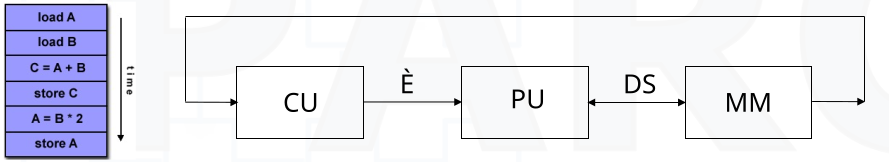
\includegraphics[width=0.7\linewidth]{img/sisd}
		\caption{Single Istruction Single Data.}
		\label{fig:sisd}
	\end{figure}
	\item SIMD (Single Instruction Multiple Data): tutte le unità di elaborazione eseguono la stessa istruzione in ogni dato ciclo di clock; ogni unità di elaborazione può operare su un dato diverso;
	\begin{figure}[th]
		\centering
		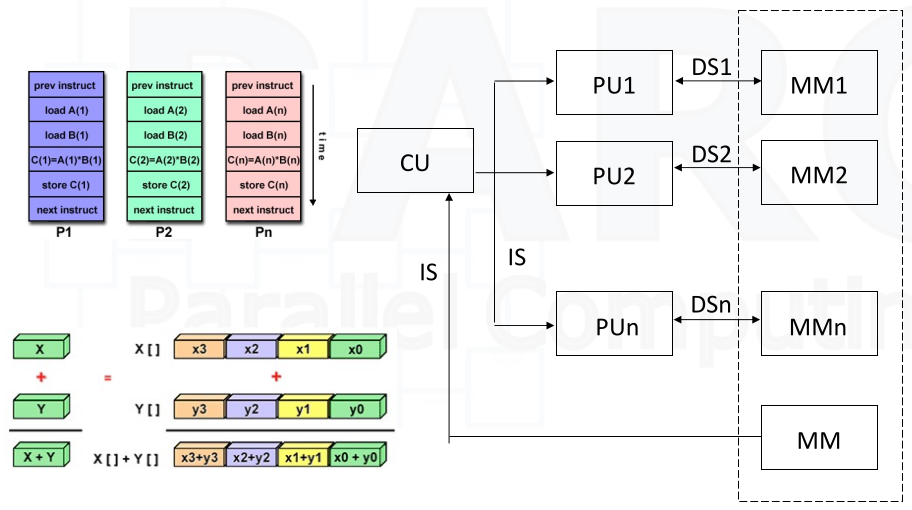
\includegraphics[width=0.7\linewidth]{img/simd}
		\caption{Single Istruction Multiple Data.}
		\label{fig:simd}
	\end{figure}

	\item MISD (Multple Instruction Single Data): un singolo flusso di dati viene immesso in più unità di elaborazione che opera sui dati in modo indipendente tramite flussi di istruzioni indipendenti. Sono esistiti pochi esempi reali di questa classe di computer paralleli;
	\begin{figure}[th]
		\centering
		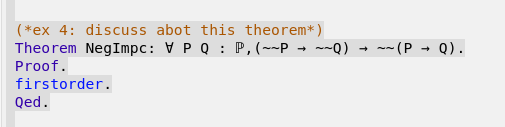
\includegraphics[width=0.7\linewidth]{img/misd}
		\caption{Multiple Instruction Single Data.}
		\label{fig:misd}
	\end{figure}

	\item MIMD (Multple Instruction Multple Data): è il tipo più comune di computer parallelo; ogni processore può eseguire un flusso di istruzioni diverso e lavorare con un flusso di dati diverso. L'esecuzione può essere sincrona o asincrona, deterministica o non deterministica.
\end{enumerate}
\subsection{Terminologia delle architetture parallele}

	\begin{longtable}{|m{0.28\linewidth}|m{0.62\linewidth}|}
		\hline
		\textbf{Termine} & \textbf{Significato}
		\\
		\hline
		\textbf{Task} & È un'unità di esecuzione o di lavoro di un programma o di un sottoprogramma.
		\\
		\hline
		\textbf{Task parallelo}& È un task che può essere eseguito in modo sicuro da più processori.
		\\
		\hline
		\textbf{Esecuzione seriale} & È l'esecuzione di un programma in sequenza, una dichiarazione alla volta. Nel senso più semplice questo accade su una macchina con un processore. Tuttavia, praticamente tutte le attività parallele avranno sezioni di un programma parallelo che devono essere eseguite in serie.
		\\
		\hline
		\textbf{Esecuzione parallela} & È l'esecuzione di un programma da più di un task, in cui ogni attività è in grado di eseguire la stessa o una diversa istruzione simultaneamente.
		\\
		\hline
		\textbf{Pipelining} & Suddivisione di un compito in passaggi eseguiti da diverse unità di elaborazione, con input che scorrono proprio come una catena di montaggio; un tipo di calcolo parallelo.
		\\
		\hline
		\textbf{Memoria condivisa} & Dal punto di vista strettamente hardware, descrive un'architettura informatica alla quale tutti i processori hanno accesso diretto (solitamente basato su bus) alla memoria fisica comune; dal punto di vista della programmazione, descrive un modello in cui le attività parallele hanno tutte la stessa "immagine" di memoria e possono indirizzarsi e accedervi direttamente alle stesse locazioni di memoria logiche indipendentemente da dove esiste effettivamente l memoria fisica.
		\\
		\hline
		\textbf{Multiprocessore simmetrico (SMP)} & Architettura hardware in cui più processori condividono un unico spazio di indirizzi e accedono a tutte le risorse; la computazione avviene su memoria condivisa.
		\\
		\hline
		\textbf{Memoria distribuita} & Nell'hardware, si riferisce all'accesso alla memoria basato sulla rete per la memoria fisica che non è in comune. Come modello di programmazione, le attività possono solo "vedere" logicamente la memoria della macchina locale e devono utilizzare comunicazioni per accedere alla memoria su altre macchine su cui sono in esecuzione altre attività.
		\\
		\hline
	\end{longtable}